\documentclass{article}
\usepackage{graphicx}
\usepackage{amsmath}
\usepackage{epsf}
\usepackage{color}
\usepackage[linesnumbered,ruled,vlined]{algorithm2e}
% titlepage causes separate title page
% our latex is biased off 1in vertically and horizontally
\newtheorem{theorem}{Theorem}
\setlength{\topmargin}{0.1in}
\setlength{\oddsidemargin}{0in}
\setlength{\evensidemargin}{0in}
\setlength{\headheight}{0in}
\setlength{\headsep}{0in}
\setlength{\textheight}{9in}
\setlength{\textwidth}{6.5in}
% require that floats fill 90% of a page in order for that page to be
% ``float-only''
\renewcommand{\dblfloatpagefraction}{0.9}
\renewcommand{\floatpagefraction}{0.9}
%\renewcommand{\baselinestretch}{1.2} % interline spacing
%\setlength{\parindent}{0in}
%\parskip=10pt plus2pt minus2pt
%\setlength{\unitlength}{0.1in}
%\pagestyle{empty} % no page numbering
\newenvironment{bibparagraph}{\begin{list}{}{ %
    \setlength{\labelsep}{-\leftmargin} %
    \setlength{\labelwidth}{0pt} %
    \setlength{\itemindent}{-\leftmargin} %
    \setlength{\listparindent}{0pt}}}{\end{list}}
\def\makefigure#1#2{\begin{figure}
\begin{center}
\input{#1}
\end{center}
\caption{#2}
\label{#1}
\end{figure}}

\def\limplies{\; \supset \;}
\def\land{\: \wedge \:}
\def\lor{\: \vee \:}
\def\iff{\; \equiv \;}
\def\lnot{\neg}
\def\lforall#1{\forall \: #1 \;}
\def\lexists#1{\exists \: #1 \;}
\def\glitch#1{{\tt #1}} % glitch on
%\def\glitch#1{} % glitch off
\def\comment#1{}
\def\pnil{[\;]}
\def\pif{\; \mbox{\tt :- } \;}
\def\tuple#1{$\langle #1\rangle$}
\def\mtuple#1{\langle #1\rangle}
\def\ceiling#1{\lceil #1\rceil}
\def\floor#1{\lfloor #1\rfloor}
\def\centerps#1{\begin{center}
\leavevmode
\epsfbox{#1}
\end{center}}
\def\argmax{\mathop{\rm argmax}}
\def\argmin{\mathop{\rm argmin}}
\def\grad{\nabla\!}
\def\celsius{^\circ\mbox{C}}
%\long\def\answer#1{}  % comment out for solutions
%\long\def\question#1{#1} % comment out for solutions
\long\def\answer#1{{\color {blue} {\sl #1}}}  % comment in for solution
\long\def\question#1{} % comment in for solution
\newcommand{\mb}[1]{{\mathbf{#1}}}
\def\z{{\bf z}}
\def\x{{\bf x}}
\def\w{{\bf w}}

\begin{document}
{\Large
\begin{center}
AI534 --- Written Homework Assignment 2 (45 pts) ---
\end{center}
}
%Please submit via TEACH electronically.
This assignment covers Kernel methods and Support vector machines.
\begin{enumerate}
\item (Cubic Kernels.) (8 pts)  In class, we showed that the quadratic
kernel $K(\x_i,\x_j) = (\x_i \cdot \x_j + 1)^2$ was equivalent to
mapping each $\x=(x_1,x_2)\in R^2 $ into a higher dimensional space where
\[\Phi(\x) = (x_1^2, x_2^2, \sqrt{2}x_1x_2, \sqrt{2}x_1, \sqrt{2}x_2, 1).\]
Now consider the cubic kernel $K(\x_i,\x_j) = (\x_i \cdot \x_j + 1)^3$.  What is the corresponding
$\Phi$ function?

\answer{ 

We use $x=(x_1, x_2)$ to calculate the cubic kernel $K(x_i, x_j) = (x_i \cdot x_j + 1)^3$. For example, we can apply $x_i = (x_{i1}, x_{i2})$ and $x_j = (x_{j1}, x_{j2})$ to the cubic kernel.  
\[ (x_i \cdot x_j + 1)^3 = (x_{i1}x_{j1}+x_{i2}x_{j2}+1)^3\]
\[ = x_{i1}^3x_{j1}^3 + x_{i2}^3x_{j2}^3 + 3x_{i1}x_{j1}x_{i2}^2x_{j2}^2 + 3x_{i1}^2x_{j1}^2x_{i2}x_{j2} + 3x_{i1}^2x_{j1}^2\]
\[ + 3x_{i2}^2x_{j2}^2 + 6x_{i1}x_{j1}x_{i2}x_{j2} + 3x_{i1}x_{j1} + 3x_{i2}x_{j2} + 1\] \\ 

From the calculation above, we can guess the corresponding $\Phi$ function like: \\
\[\Phi(x_i) \cdot \Phi(x_j) = (x_{i1}^3, x_{i2}^3, \sqrt{3}x_{i1}x_{i2}^2, \sqrt{3}x_{i1}^2x_{i2}, \sqrt{3}x_{i1}^2, \sqrt{3}x_{i2}^2, \sqrt{6}x_{i1}x_{i2}, \sqrt{3}x_{i1}, \sqrt{3}x_{i2}, 1) \]
\[  \cdot (x_{j1}^3, x_{j2}^3, \sqrt{3}x_{j1}x_{j2}^2, \sqrt{3}x_{j1}^2x_{j2}, \sqrt{3}x_{j1}^2, \sqrt{3}x_{j2}^2, \sqrt{6}x_{j1}x_{j2}, \sqrt{3}x_{j1}, \sqrt{3}x_{j2}, 1) \] \\

Since the product of two $\Phi$ functions should hold the cubic kernel calculation above. 
Thus, we finally get:  

\[\Phi(\textbf{x})=(x_1^3, x_2^3, \sqrt{3}x_1^2x_2, \sqrt{3}x_1x_2^2, \sqrt{3}x_1^2, \sqrt{3}x_2^2, \sqrt{3}x_1, \sqrt{3}x_2, \sqrt{6}x_1x_2, 1)\] \\
}

\item (Kernel or not). (5 pts) Suppose that $K_1$ and $K_2$ are kernels with feature maps $\phi_1$ and $\phi_2$ respectively. Is function $K(\x,\z)= c_1K_1(\x, \z)+c_2K_2(\x,\z)$ for $c_1, c_2 >0$ a kernel function?  If your answer is yes, write down the corresponding
$\phi$ in terms of $\phi_1$ and $\phi_2$. If not, provide a proof or explain why.
 
\answer{Your answer goes here.}

\item Kernelizing Logistic Regression (10 pts) 
For this problem you will follow the example of kernelizing perceptron, to kernelize the logistic regression shown below.

\begin{minipage}{0.8\linewidth}    
\begin{algorithm}[H]
\SetAlgoLined
\KwIn{$\{(\x_i,y_i)_{i=1}^N\}$(training data), $\gamma$(learning rate)}
\KwOut{learned weight vector $\w$}

 Initialize $\w=\mb{0}$\;
 \While{not converged}{
    \For{$i=1,...,N$}{ $\w\leftarrow \w + \gamma(y_i-\sigma(\w^T\x_i))\x_i$ 
  }
  
 }
 \caption{Stochastic gradient descent for logistic regression}
\label{alg-l2}
\end{algorithm}
\end{minipage}

Specifically, please:
\begin{enumerate}
    \item (4 pts) Argue that the solution $\w^*$ for logistic regression can be expressed as the weighted sum of training examples (similar to slide 8 of the kernel methods lecture)\\
    \answer{Your answer goes here.}
    \item (6 pts) Modify the following stochastic gradient descent algorithm logistic regression algorithm to kernelize it. (Hint: similar to the bottom algorithm on slide 14 of the kernel method lecture, but instead of counter, you will learn a continuous weights for $\alpha$'s)\\
    \answer{    
Your answer goes here.
}
\end{enumerate}
\newpage
\item (Hard margin SVM) (8 pts) Apply linear SVM without soft margin to the following problem.
\begin{center}
\begin{figure}[h]
    \centering
    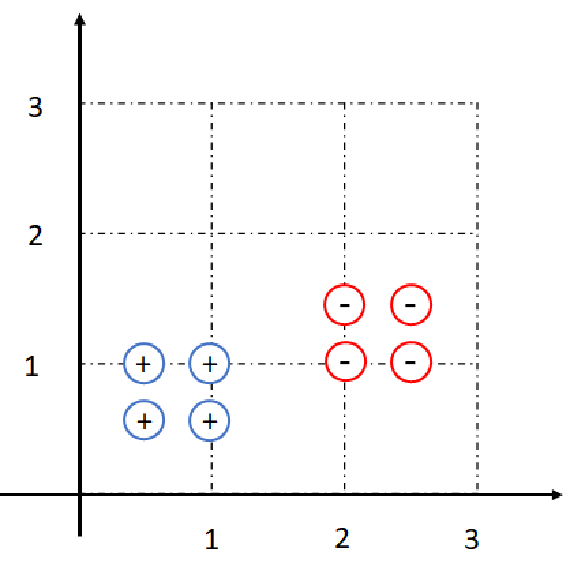
\includegraphics[width=0.5\linewidth]{svm.pdf}
    \caption{ }
    \label{fig:enter-label}
\end{figure}
\end{center}
\begin{itemize} \item[a.] (3pts) Please mark out the support vectors, the decision boundary ($w_1x_1+w_2x_2 +b =0$) and $w_1x_1+w_2x_2+b =1$ and $w_1x_1+w_2x_2+b =-1$. You don't need to solve the optimization problem for this, you should be able to eyeball the solution and find the linear separator with the largest margin.

\answer{Your answer goes here.}
\item[b.] (5 pts) Please solve for $w_1, w_2$ and $b$ based on the support vectors you identified in (a). Hint: the support vectors would have functional margin = 1. \\
\answer{Your answer goes here.}
\end{itemize}
\item $L_2$ SVM (14 pts) \\
Given a set of training examples $\{(\x_i, y_i)\}_{i=1}^N$, where $y_i\in \{1, -1\}$ for all $i$. The following is the primal formulation of $L_2$ SVM, a variant of the standard SVM obtained by squaring the slacks.
\begin{align*}
\min_{\w, b, \xi} \mbox{ }& \frac{1}{2}\w^T\w+c\sum_{i=1}^N \xi_i^2 \\
\mbox{s.t. } & y_i(\w^T\x_i+b)\geq 1-\xi_i \mbox{,   } i \in \{1,\cdots,N\}\\
 & \xi_i\geq 0, \mbox{  }  i\in \{1,\cdots,N\}
\end{align*}

\begin{itemize}
\item [a.] (3pts) Show that removing the second constraint $\xi_i\geq 0$ will not change the solution to the problem. In other words, let $(\w^*, b^*, {\bf \xi}^*)$ be the optimal solution to the problem without this set of constraints, show that ${\bf \xi}_i^* \geq 0$ must be true, $\forall i\in\{1,\cdots,N\} $. ( Hint: use proof by contradiction by assuming that there exists some $\xi_i^*<0$.)\\
\answer{Your answer goes here}
\item [b.] (3 pts) After removing the second set of constraints, we have a simpler problem with only one set of constraints. Now provide the lagrangian of this new problem.\\
\answer{Your answer goes here}
\item [c.] (8pts) Derive the dual of this problem. How is it different from the standard SVM with hinge loss? Which formulation is more sensitive to outliers?\\
\answer{Your answer goes here
}

\end{itemize}
\end{enumerate}

\end{document}
